\level{2}{Applicazione Android}
	\begin{figure}[H]\centering
        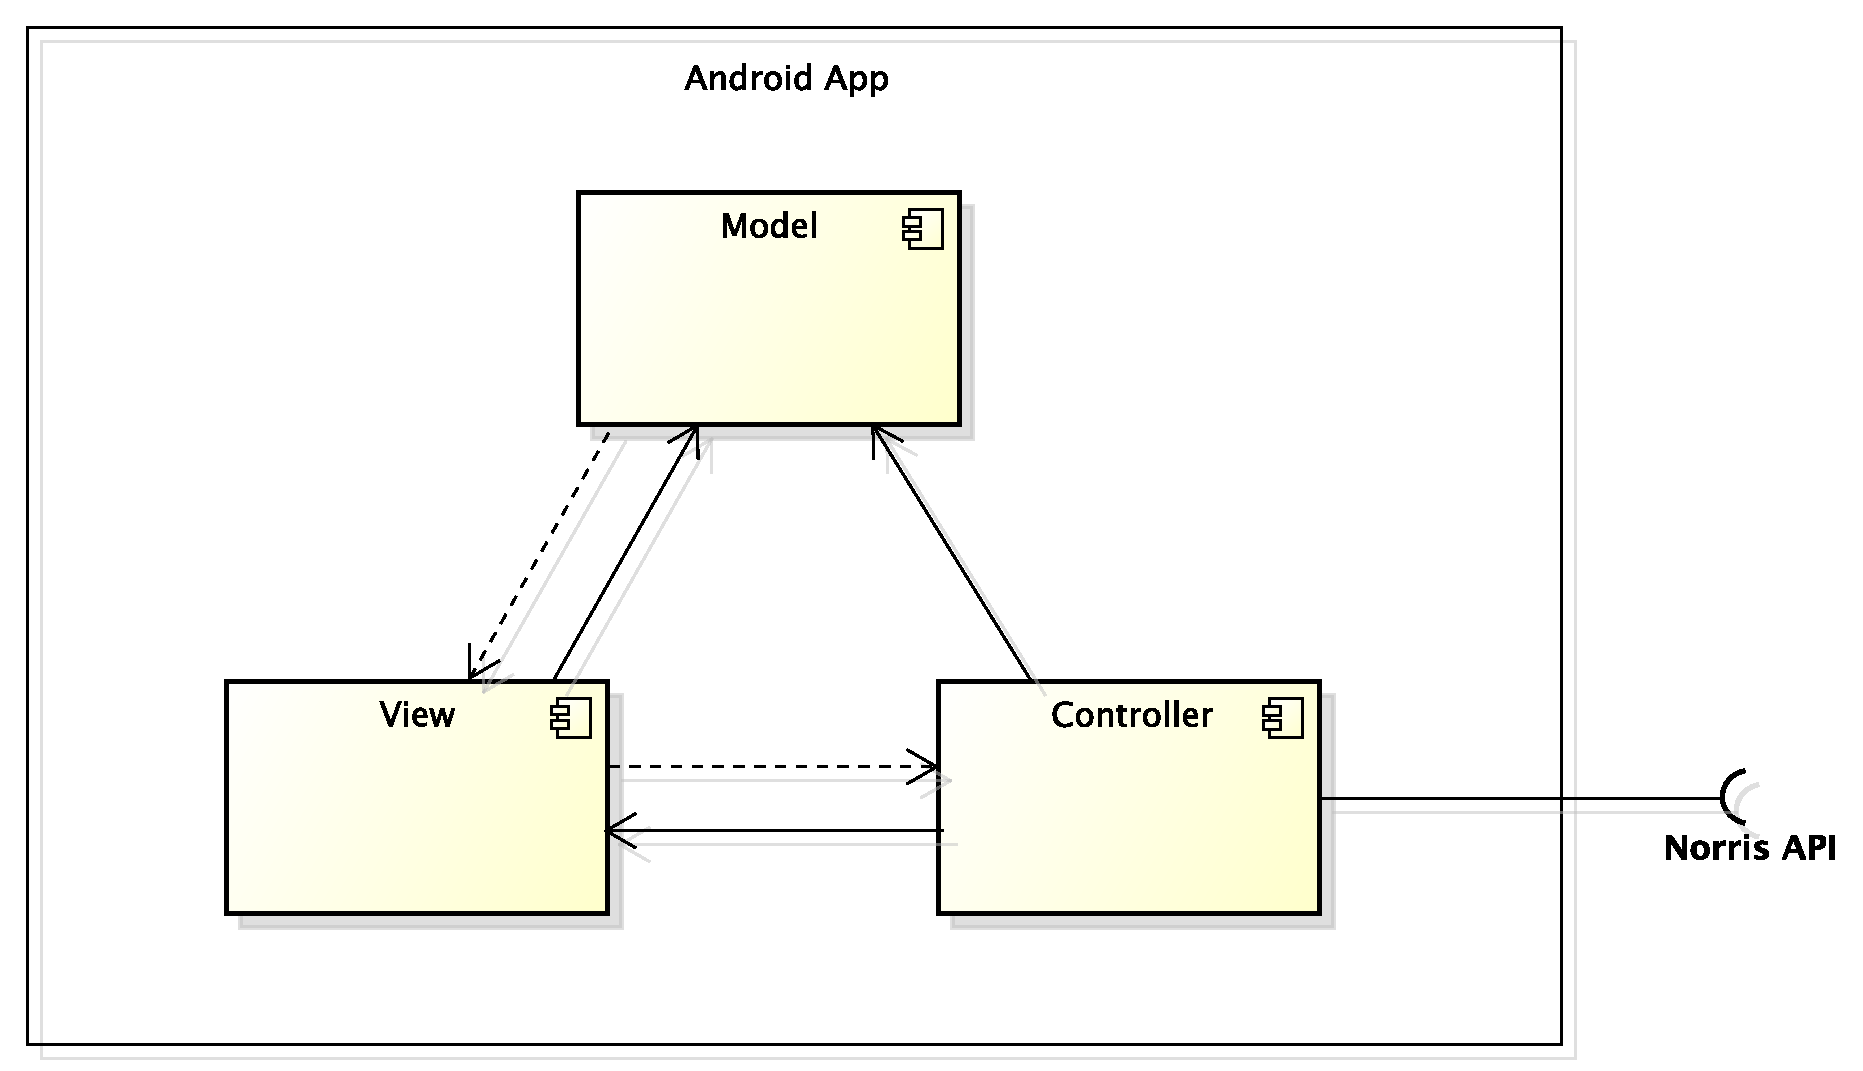
\includegraphics[width=\textwidth]{SpecificaTecnica/Pics/ComponentiApplicazione}
        \caption{Diagramma delle componenti dell'Applicazione Android}
    \end{figure}
    \level{3}{Descrizione delle componenti dell'Applicazione}
    	\level{4}{Model} 
            Il Model è la componente che rappresenta l'astrazione dei grafici visualizzati nell'applicazione. In essa sono contenuti i dati riguardanti i grafici, assieme alle relative impostazioni. In particolare sono presenti i modelli di tutte le tipologie di chart implementati da \insglo{Norris}. Il Model fornisce per ciascuna tipologia di grafico i metodi per inserire i dati e configurare alcune impostazioni. Si occupa inoltre di gestire gli aggiornamenti dei grafici mantenendo una comunicazione con Norris tramite un canale websocket e di richiedere un chart utilizzando le \insglo{API} esterne di \insglo{Norris}. Infine nel Model sono memorizzate tutte le informazioni inerenti lo stato della sessione con l'istanza di Norris contenente i grafici che si vogliono visualizzare con l'applicazione.
    
       \level{4}{View}
        La View è il componente che rappresenta le varie UI dell'applicazione. In tale componente potrebbero esser sollevati degli eventi scatenati dall'utente attraverso User Gesture. Questi eventi vengono mandati al Presenter che deciderà come comportarsi.
       \level{4}{Presenter}
        Questo componente ha il compito di gestire tutto il controllo dell'applicazione. Le operazioni che esso gestisce sono riassunte nel seguente elenco:
        	\begin{itemize}
        		\item creazione del modello qualora questo sia necessario;
        		\item utilizzo delle \insglo{API} esterne di \insglo{Norris} (Autenticazione, Richiesta della lista);
        		\item interpretazione dei pacchetti ricevuti dal \insglo{server} contenenti i dati delle richieste \insglo{API} effettuate;
                \item chiede al modello di attivare gli aggiornamenti per un certo grafico.
        		\item interpretazione dei pacchetti di aggiornamento;
        		\item richiesta al modello di aggiornare il proprio stato;
        		\item modifica della view;
        		\item avvio delle varie \insglo{activity} dell'applicazione;
        		\item gestione delle \insglo{gesture} dell'utente.
        \end{itemize}
    \level{3}{Descrizione delle interazioni tra le componenti}
    	Le interazioni tra i componenti sono rappresentati con una freccia tratteggiata.\\
    	Riportiamo di seguito la descrizione di ogni interazione.

    	\level{4}{View - Presenter}
        In seguito all'esecuzione di una \insglo{gesture} da parte dell'utente, la View notifica il Presenter tramite l'emissione dell'evento opportuno. Il Presenter si occupa quindi di gestire quest'ultimo. Questa interazione si verifica in particolare quando l'utente seleziona un item della lista dei grafici presenti nell'istanza di \insglo{Norris} richiesta.

        \level{4}{Presenter - View}
        Tale interazione rappresenta la selezione di un'activity modifica tale view. Ciò avviene ad ogni necessità di cambiare \insglo{Activity} e/o quando deve modificare o inizializare la view.

        \level{4}{Presenter - Model}
        Il Presenter richiede al Model di modificare il proprio stato. Ciò avviene per esempio subito dopo l'utilizzo dell'\insglo{API} esterna di \insglo{Norris} per richiedere un grafico o in seguito all'arrivo di un pacchetto di aggiornamento.

        \level{4}{Model - Presenter}
        Tale interazione rappresenta l'invio dei valori del chart provenienti dal server norris oppure, se nel Model è stato attivato il socket per l'aggiornamento, rappresenta la notifica del Model verso il Presenter di avvenuta modifica del chart sul server.

        
    \level{3}{Design pattern utilizzati}
    Riportiamo di seguito i pattern architetturali utilizzati nella progettazione delle componenti dell'applicazione Android.
        \level{4}{Model View Presenter}
        Model-View-Presenter (\insglo{MVP}) è un \insglo{pattern} architetturale utilizzato per separare il codice in blocchi di funzionalità ben distinte.\\
        Per la descrizione del \insglo{pattern} e dei vantaggi derivanti dalla sua applicazione si rimanda all'appendice \nameref{app:MVP}.
        \level{5}{Contesto di utilizzo}
        L'\insglo{MVP} viene utilizzato per dividere le classi dell'applicazione \insglo{Android} in tre grandi componenti:
        \begin{itemize}
        \item Model;
        \item View;
        \item Presenter;
        \end{itemize}

